% Generative adversarial network (GAN) architecture.
% Adapted from https://github.com/PetarV-/TikZ/tree/master/Generative%20adversarial%20network.
% A GAN has two parts. The discriminator $D$ acts as a classifier that learns to distinguish fake data produced by the generator $G$ from real data. $G$ incurs a penalty when $D$ detects implausible results. This signal is backpropagated through the generator weights such that $G$ learns to produce more realistic samples over time, eventually fooling the discriminator if training succeeds.

\documentclass[tikz]{standalone}

\usepackage{mathtools}

\usetikzlibrary{calc,positioning}

\colorlet{myred}{red!80!black}
\colorlet{myblue}{blue!80!black}
\colorlet{mybluee}{myblue!80!black}
\colorlet{mygreen}{green!60!black}
\colorlet{myorange}{orange!70!red!60!black}
\colorlet{mydarkred}{red!30!black}
\colorlet{mydarkblue}{blue!40!black}
\colorlet{mydarkgreen}{green!30!black}



\begin{document}
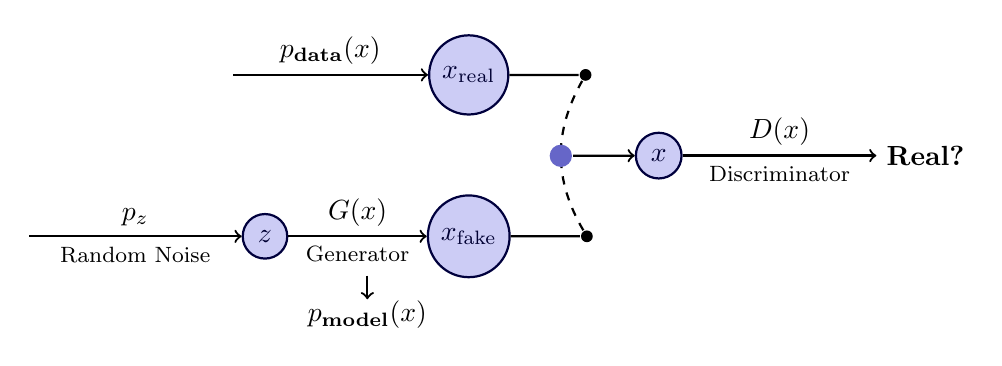
\begin{tikzpicture}[
    ->, thick,
    % node/.style={circle, fill=teal!60},
    node/.style={circle, blue!20!black,draw=myblue!30!black,fill=myblue!20},
    label/.style={below, font=\footnotesize},
  ]

  \node[node] (zin) {$z$};
  \node[node, right=5em of zin] (fake) {$x_\text{fake}$};
  \draw (zin) -- node[above] {$G(x)$} node[label] {Generator} (fake);
  \node at (1.3,-1) {$p_\text{\textbf{model}}(x)$};
  \draw (1.3,-0.5) -- node[above] {} node[label] {} (1.3,-0.8);

  \draw[<-] (zin) -- node[above] {$p_z$} node[label] {Random Noise} ++(-3,0);
  \node[node, above=of fake] (real) {$x_\text{real}$};
  \draw[<-] (real) -- node[above] {$p_\text{\textbf{data}}(x)$} ++(-3,0);
  \node[node, right=6em of fake] (D) at ($(fake)!0.5!(real)$) {$x$};
  \node[right=7em of D] (out) {\textbf{Real?}};
  \draw (D) -- node[above] {$D(x)$} node[label] {Discriminator} (out);

  \coordinate[right=2.5em of fake, circle, fill, inner sep=0.15em] (pt1);
  \coordinate[right=2.5em of real, circle, fill, inner sep=0.15em] (pt2);

  \draw[-, dashed] (pt1) edge[bend left] coordinate[circle, fill=mybluee!60, inner sep=1mm] (pt3) (pt2);
  \draw (fake) -- (pt1) (real) -- (pt2) (pt3) -- (D);

\end{tikzpicture}
\end{document}